\section{Resultados}

%---------------------------------------------------------------
\subsection{Visualización en el dominio del tiempo y de la frecuencia de una onda sinusoidal con el programa VisSim}

\begin{center}
    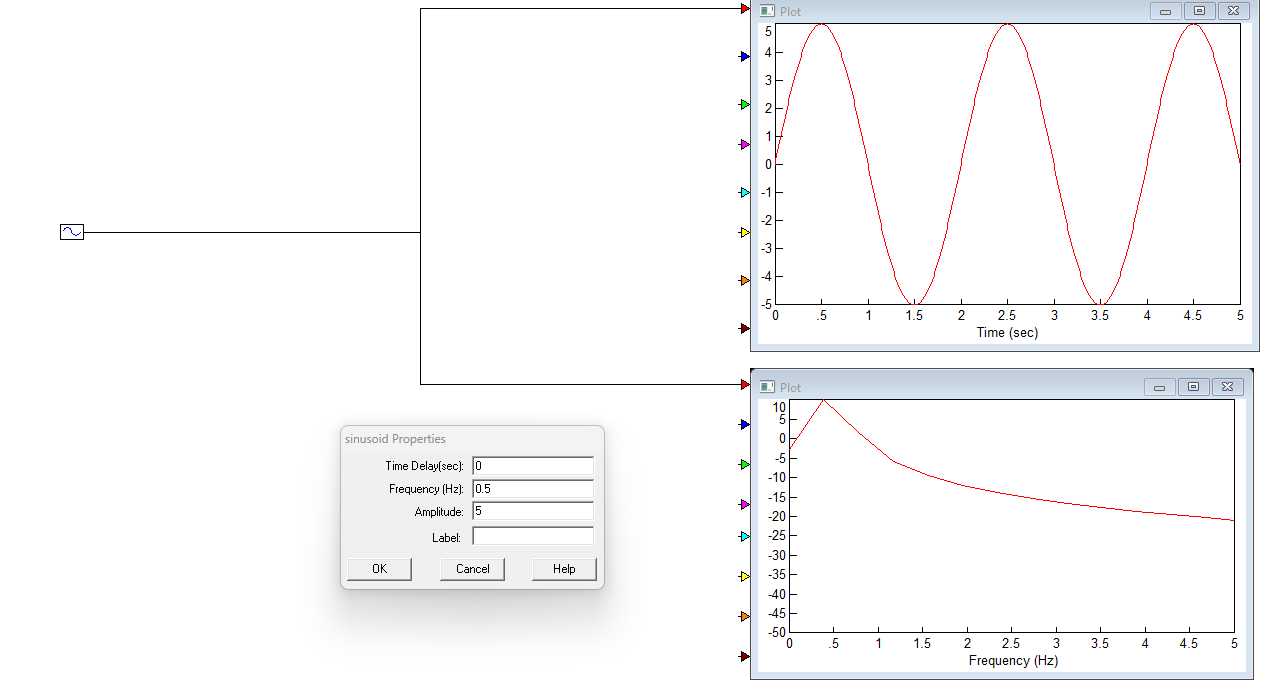
\includegraphics[width=0.8\linewidth]{Imagenes/parte-1-señal-sinusoidal.png}
    \captionof{figure}{Señal sinusoidal visualizada en el dominio del tiempo y la frecuencia mediante VisSim.}
    \label{fig:parte1-sinusoidal}
\end{center}


%---------------------------------------------------------------
\subsection{Construcción aproximada de las formas de las señales, con las primeras cinco componentes espectrales de su serie de Fourier}

\begin{center}
    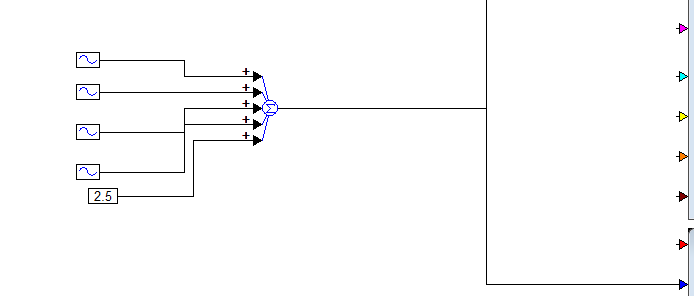
\includegraphics[width=0.8\linewidth]{Imagenes/parte-2-sistema.png}
    \captionof{figure}{Esquema del sistema para la construcción de señales mediante componentes espectrales.}
    \label{fig:parte2-sistema}
\end{center}

\begin{center}
    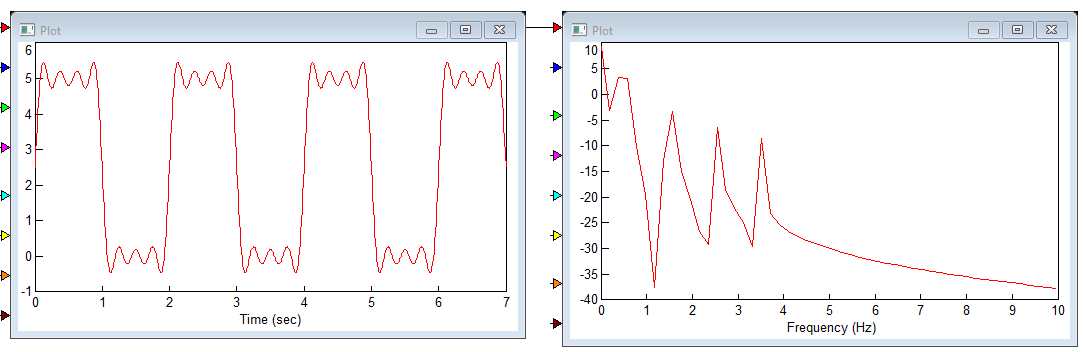
\includegraphics[width=0.8\linewidth]{Imagenes/parte-2-onda-cuadrada.png}
    \captionof{figure}{Construcción de una onda cuadrada a partir de sus primeras cinco componentes de Fourier.}
    \label{fig:parte2-cuadrada}
\end{center}

\begin{center}
    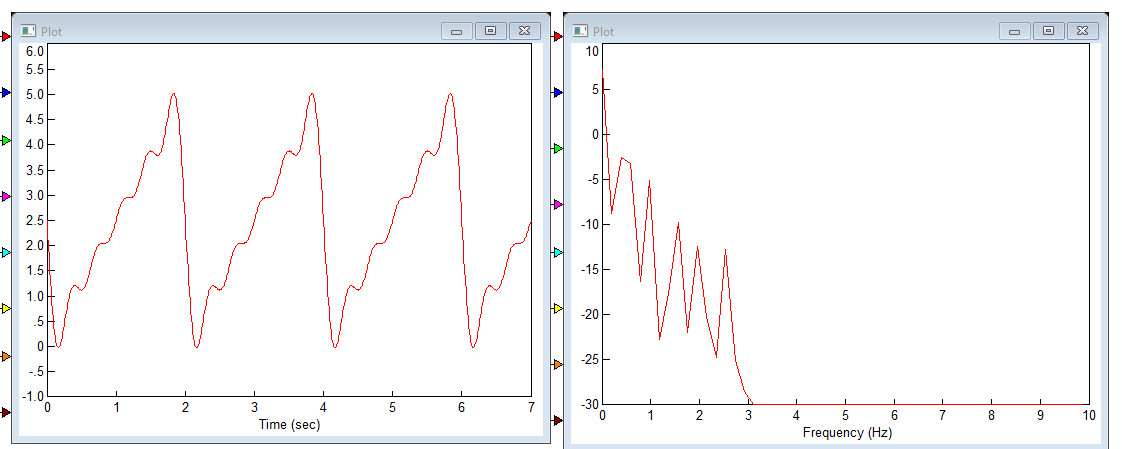
\includegraphics[width=0.8\linewidth]{Imagenes/parte-2-onda-diente-de-sierra.png}
    \captionof{figure}{Construcción de una onda diente de sierra a partir de sus primeras cinco componentes de Fourier.}
    \label{fig:parte2-diente-sierra}
\end{center}

\begin{center}
    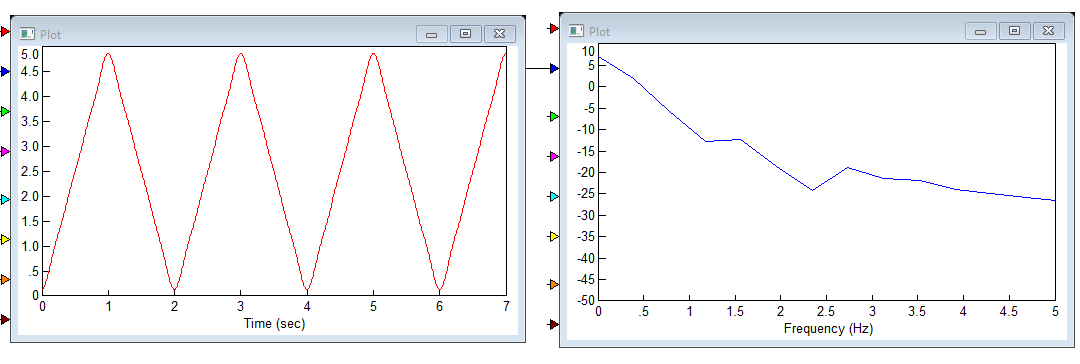
\includegraphics[width=0.8\linewidth]{Imagenes/parte-2-triangular.png}
    \captionof{figure}{Construcción de una onda triangular a partir de sus primeras cinco componentes de Fourier.}
    \label{fig:parte2-triangular}
\end{center}

%---------------------------------------------------------------
\subsection{Comparación con el generador de forma de onda}

\begin{center}
    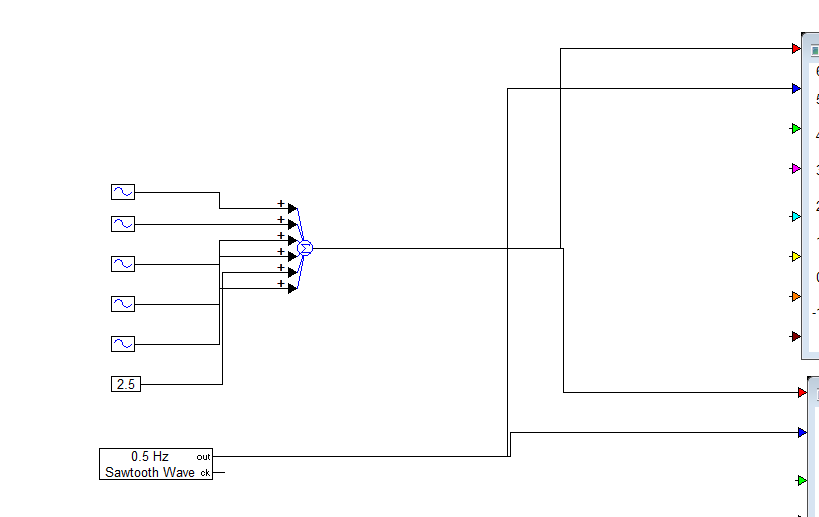
\includegraphics[width=0.8\linewidth]{Imagenes/parte-3-sistema.png}
    \captionof{figure}{Sistema para la comparación de señales con el generador de funciones.}
    \label{fig:parte3-sistema}
\end{center}

\begin{center}
    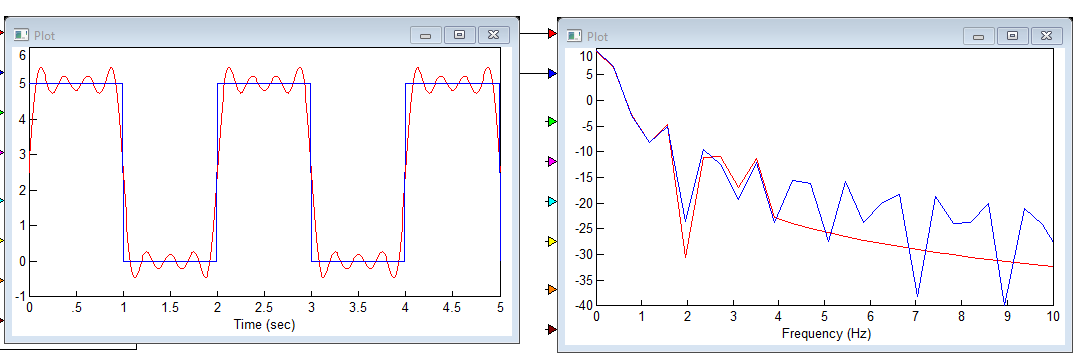
\includegraphics[width=0.8\linewidth]{Imagenes/parte-3-cuadrada-comparacion.png}
    \captionof{figure}{Comparación de la señal cuadrada generada vs la teórica.}
    \label{fig:parte3-cuadrada-comp}
\end{center}

\begin{center}
    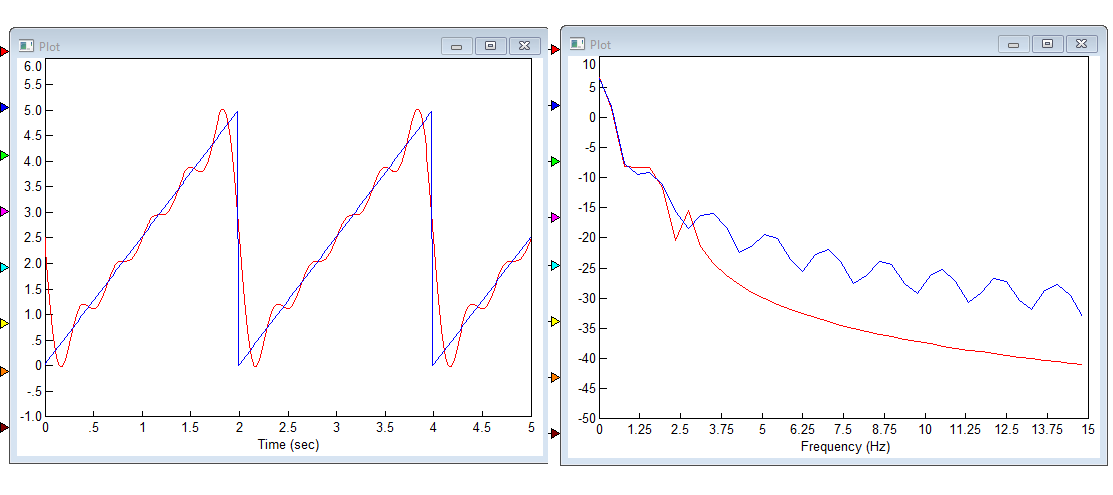
\includegraphics[width=0.8\linewidth]{Imagenes/parte-3-diente-de-sierra-comparacion.png}
    \captionof{figure}{Comparación de la señal diente de sierra generada vs la teórica.}
    \label{fig:parte3-diente-sierra-comp}
\end{center}

\begin{center}
    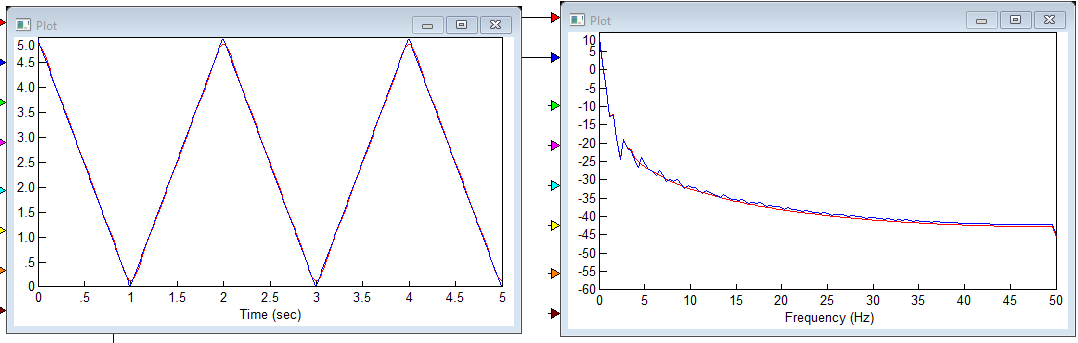
\includegraphics[width=0.8\linewidth]{Imagenes/parte-3-triangular-comparacion.png}
    \captionof{figure}{Comparación de la señal triangular generada vs la teórica.}
    \label{fig:parte3-triangular-comp}
\end{center}

%---------------------------------------------------------------
\subsection{Distorsión de amplitud y distorsión de retardo}

\begin{center}
    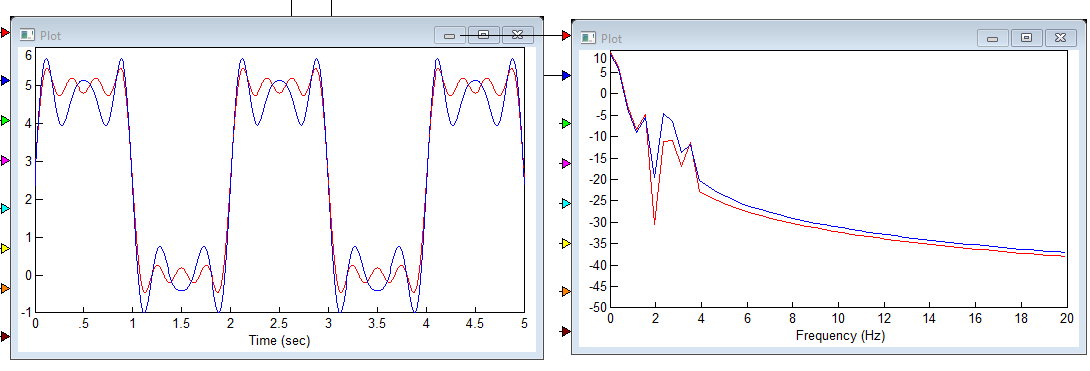
\includegraphics[width=0.8\linewidth]{Imagenes/parte-4-distorsion-de-amplitud.png}
    \captionof{figure}{Efecto de la distorsión de amplitud en la señal recibida.}
    \label{fig:parte4-distorsion-amplitud}
\end{center}

\begin{center}
    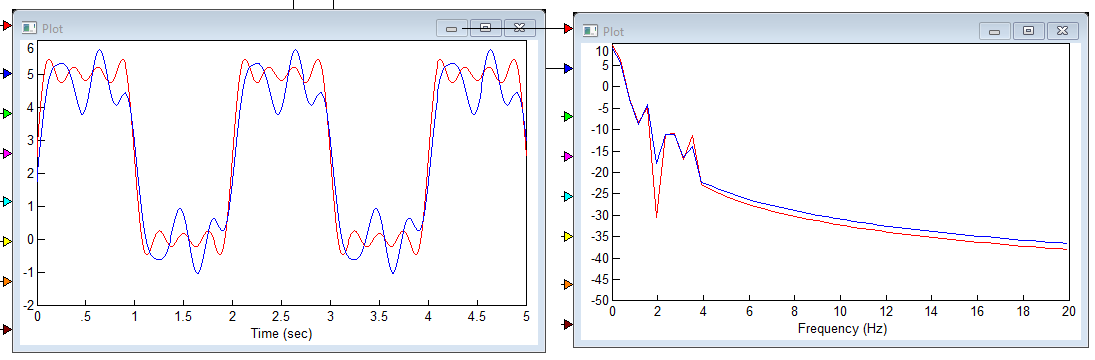
\includegraphics[width=0.8\linewidth]{Imagenes/parte-4-distorsion-por-retardo.png}
    \captionof{figure}{Efecto de la distorsión por retardo en la señal recibida.}
    \label{fig:parte4-distorsion-retardo}
\end{center}

\begin{center}
    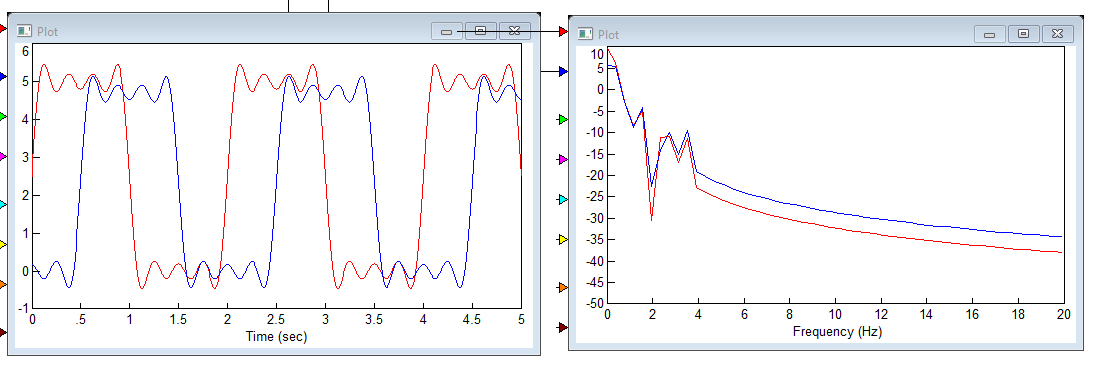
\includegraphics[width=0.8\linewidth]{Imagenes/parte-4-retardo-homogeneo.png}
    \captionof{figure}{Señal con retardo homogéneo sin distorsión significativa.}
    \label{fig:parte4-retardo-homogeneo}
\end{center}
